% Build: module load texlive/20240312-GCC-13.3.0 && latexmk -pdf rebuild_talk.tex

\documentclass[11pt,aspectratio=169]{beamer}

% ---------------------------------------------------------------------------
% Look: plain beamer, Yale colours
% ---------------------------------------------------------------------------
\usetheme{default}
\usefonttheme{professionalfonts}
\setbeamertemplate{navigation symbols}{}

\definecolor{yaleblue}{HTML}{00356B}
\definecolor{yalemid}{HTML}{286DC0}
\definecolor{yalelight}{HTML}{63AAFF}
\definecolor{yalegrey}{HTML}{4A4A4A}
\definecolor{yalelightgrey}{HTML}{DDDDDD}

\setbeamercolor{structure}{fg=yaleblue}
\setbeamercolor{normal text}{fg=black}
\setbeamercolor{frametitle}{fg=yaleblue}
\setbeamercolor{title}{fg=yaleblue}
\setbeamercolor{alerted text}{fg=yalemid}
\setbeamercolor{block title}{fg=white,bg=yaleblue}
\setbeamercolor{block body}{bg=yalelightgrey!40}

\setbeamerfont{frametitle}{series=\bfseries,size=\large}
\setbeamerfont{title}{series=\bfseries,size=\Large}

\setbeamertemplate{itemize items}[circle]
\setbeamertemplate{blocks}[rounded][shadow=false]

% A thin blue rule under each frame title
\setbeamertemplate{frametitle}{%
  \vspace*{0.6em}%
  \usebeamerfont{frametitle}\usebeamercolor[fg]{frametitle}\insertframetitle\par
  \vspace*{-0.2em}{\color{yaleblue}\rule{\textwidth}{0.6pt}}%
}

% Footer: short title on the left, slide number on the right
\setbeamertemplate{footline}{%
  \hspace*{1.2em}{\color{yalegrey}\scriptsize\insertshorttitle}%
  \hfill{\color{yalegrey}\scriptsize\insertframenumber}\hspace*{1.2em}%
  \vspace*{0.6em}%
}

% ---------------------------------------------------------------------------
% Packages
% ---------------------------------------------------------------------------
\usepackage[T1]{fontenc}
\usepackage{lmodern}
\usepackage{booktabs}
\usepackage{graphicx}
\usepackage{amsmath}
\usepackage{tikz}
\usetikzlibrary{positioning,arrows.meta,calc}
\usepackage{pgfplots}
\pgfplotsset{compat=1.18}
\graphicspath{{figures/}}

% Diagram styles
\tikzset{
  tok/.style={draw=yaleblue, rounded corners=2pt, font=\small, inner sep=4pt,
              minimum height=0.65cm},
  blank/.style={tok, fill=yalelight!35, font=\small\bfseries},
  box/.style={draw=yaleblue, rounded corners=2pt, font=\scriptsize, align=center,
               text width=2.1cm, minimum height=1.1cm, inner sep=3pt},
  arr/.style={-{Stealth[length=5pt]}, yaleblue, thick},
  cF/.style={fill=yaleblue},
  cP/.style={fill=yalelight!60},
  cN/.style={fill=white},
}

\pgfplotsset{colormap={yalemap}{color=(white) color=(yalelight) color=(yaleblue)}}


% Distribution maps (slides on pretraining and post-training): a smooth 2D
% density from Gaussian bumps g, shaded white to Yale blue.
\pgfplotsset{sentencemap/.style={view={0}{90}, width=6.6cm, height=5.4cm,
    xmin=-3, xmax=3, ymin=-3, ymax=3, ticks=none, colormap name=yalemap,
    axis line style={yalegrey}, clip=false,
    /pgf/declare function={g(\x,\y,\a,\b,\s) = exp(-((\x-\a)^2 + (\y-\b)^2)/(2*\s^2));}}}

% Four labelled points on a distribution map, at fixed positions:
% #1 top left, #2 top right, #3 bottom right, #4 bottom left (the unrealistic one)
\newcommand{\maplabels}[4]{%
  \begin{scope}[every node/.style={font=\tiny, fill=white, fill opacity=0.8,
        text opacity=1, inner sep=1.5pt, rounded corners=1pt, align=left}]
    \fill[black] (axis cs:-1.6,1.2,5) circle (1.2pt);
    \node[anchor=south west] at (axis cs:-1.7,1.3,5) {#1};
    \fill[black] (axis cs:1.4,1.3,5) circle (1.2pt);
    \node[anchor=north, align=center] at (axis cs:1.4,1.2,5) {#2};
    \fill[black] (axis cs:1.5,-1.5,5) circle (1.2pt);
    \node[anchor=north, align=center] at (axis cs:1.5,-1.6,5) {#3};
    \fill[black] (axis cs:-2.2,-2.4,5) circle (1.2pt);
    \node[anchor=south west] at (axis cs:-2.2,-2.3,5) {#4};
  \end{scope}}

\newcommand{\recordlabels}{\maplabels{married, 38,\\ two children}{age 81, Social\\ Security \$31k}{age 70, \$400k saved,\\ \$2k interest (0.5\%)}{age 9, wages \$300k}}

% Training slide. Cells sit at column #1, row #2 of a picture with x=1.5cm, y=0.85cm.
\tikzset{
  cell/.style={tok, minimum width=1.38cm, minimum height=0.7cm, font=\scriptsize},
  hid/.style={blank, minimum width=1.38cm, minimum height=0.7cm, font=\scriptsize\bfseries},
  absent/.style={cell, draw=yalelightgrey, fill=yalelightgrey!50, text=yalegrey},
}
\newcommand{\cellv}[3]{\node[cell] at (#1,-#2) {#3};}          % a visible value
\newcommand{\cellh}[2]{\node[hid] at (#1,-#2) {?};}            % a hidden cell
\newcommand{\cella}[2]{\node[absent] at (#1,-#2) {--};}        % not in this source
% A guessed distribution: #3 the bar heights (tallest = 1), #4 the true bar
% (0 = truth not shown yet), #5 the true value
\newcommand{\cellg}[5]{%
  \node[hid] at (#1,-#2) {};
  \foreach \hgt [count=\k] in {#3} {
    \ifnum\k=#4 \def\barcol{yaleblue}\else\def\barcol{yalemid!40}\fi
    \fill[\barcol] ($(#1,-#2)+(-0.75cm+\k*0.15cm,-0.27cm)$) rectangle ++(0.1cm,\hgt*0.5cm);
  }
  \ifnum#4>0 \node[font=\tiny, text=yaleblue] at ($(#1,-#2)+(0.4cm,0)$) {#5};\fi
}
% The network strip under the table: idle, guess (arrows on), or update (weights lit)
\newcommand{\trainnet}[1]{%
  \begin{scope}[shift={(5,-5.5)}, x=1cm, y=1cm]
    \def\mode{#1}\def\upd{update}\def\idle{idle}
    \ifx\mode\upd \def\wcol{yalemid}\def\wth{0.9pt}\else \def\wcol{yalelightgrey}\def\wth{0.4pt}\fi
    \foreach \a in {-0.5,-0.17,0.17,0.5} \foreach \b in {-0.5,-0.17,0.17,0.5} {
      \draw[\wcol, line width=\wth] (-0.8,\a) -- (0,\b);
      \draw[\wcol, line width=\wth] (0,\a) -- (0.8,\b);
    }
    \foreach \lx in {-0.8,0,0.8} \foreach \ly in {-0.5,-0.17,0.17,0.5}
      \fill[yaleblue] (\lx,\ly) circle (2.2pt);
    \ifx\mode\idle\else
      \draw[arr] (-3.2,0) -- (-1.1,0);
      \node[font=\scriptsize, anchor=south] at (-2.15,0.05) {visible cells};
      \draw[arr] (1.1,0) -- (2.9,0);
      \node[font=\scriptsize, anchor=south] at (2.0,0.05) {a guess for each ?};
    \fi
    \ifx\mode\upd \node[font=\scriptsize, text=yalemid, anchor=north] at (0,-0.6) {adjust the weights}; \fi
  \end{scope}}

% 100 squares, 10 by 10, at #1: the first #2 dark, the next #3 light, the rest
% empty; #4 a caption underneath
\newcommand{\waffle}[4]{%
  \begin{scope}[shift={(#1)}]
    \foreach \n in {0,...,99} {
      \pgfmathtruncatemacro{\col}{mod(\n,10)}
      \pgfmathtruncatemacro{\row}{div(\n,10)}
      \pgfmathtruncatemacro{\light}{#2+#3}
      \ifnum\n<#2 \def\wf{yaleblue}\else\ifnum\n<\light \def\wf{yalelight!70}\else\def\wf{white}\fi\fi
      \filldraw[fill=\wf, draw=yalegrey!60] (\col*0.32, -\row*0.32) rectangle ++(0.28,0.28);
    }
    \node[font=\small, anchor=north] at (1.58,-3.05) {#4};
  \end{scope}}

% Small grey note at the bottom of a slide
\newcommand{\slidenote}[1]{\par\vfill{\scriptsize\color{yalegrey}#1}}

% ---------------------------------------------------------------------------
% Title
% ---------------------------------------------------------------------------
\title{Using deep learning to generate synthetic tax records}
\author{John Ricco}
\institute{The Budget Lab at Yale}
\date{October 28, 2026}

\begin{document}

\begin{frame}[plain,noframenumbering]
  \titlepage
\end{frame}

% ===========================================================================
% 1. The job
% ===========================================================================

\begin{frame}{What Tax-Simulator needs}
  \centering
  \small
  \begin{tabular}{rrrrrrrr}
    \toprule
    Married & Dependents & Age & Wages & Interest & Cap.\ gains & Net worth & Weight \\
    \midrule
    yes & 2 & 44 & \$142,000 & \$310   & \$5,200  & \$610,000   & 812   \\
    no  & 0 & 27 & \$38,000  & \$0     & \$0      & \$9,000     & 1,404 \\
    yes & 0 & 71 & \$0       & \$4,900 & \$61,000 & \$2,400,000 & 655   \\
    \multicolumn{8}{c}{\dots\ about 200 million more} \\
    \bottomrule
  \end{tabular}

  \vspace{1.5em}
  \normalsize
  \begin{itemize}
    \item Realistic records: the variables go together the way they do in life
    \item The right totals for the year
    \item Every year, 2015 to 2060
  \end{itemize}
  \slidenote{Made-up records.}
\end{frame}

% ===========================================================================
% 2. The problem
% ===========================================================================

\begin{frame}{The information is scattered}
  \centering
  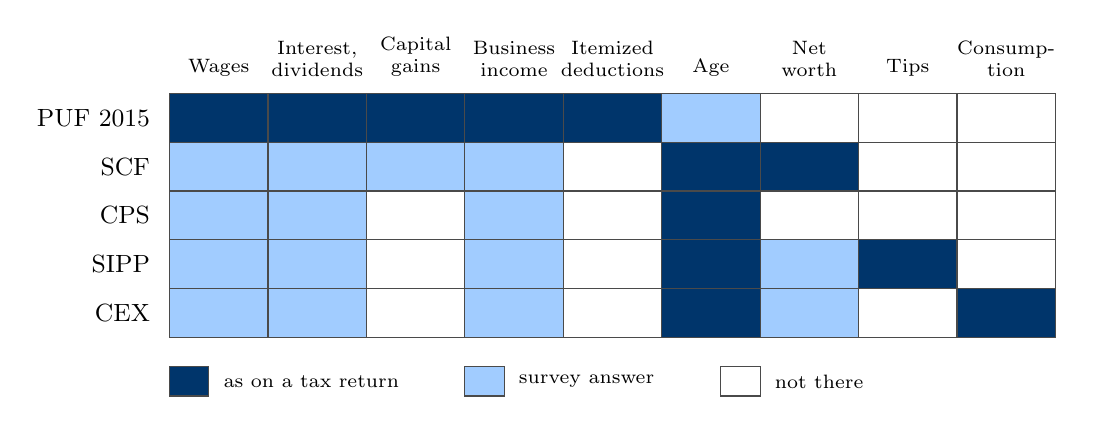
\begin{tikzpicture}[x=1.25cm, y=0.62cm]
    % column labels
    \foreach \lab [count=\i] in {Wages, {Interest,\\dividends}, {Capital\\gains},
        {Business\\income}, {Itemized\\deductions}, Age, {Net\\worth}, Tips, {Consump-\\tion}} {
      \node[font=\scriptsize, align=center, anchor=south] at (\i-0.5, 0.15) {\lab};
    }
    % rows: F = on a tax return, P = survey answer, N = not there
    \foreach \lab/\codes [count=\j] in {
        PUF 2015/{cF,cF,cF,cF,cF,cP,cN,cN,cN},
        SCF/{cP,cP,cP,cP,cN,cF,cF,cN,cN},
        CPS/{cP,cP,cN,cP,cN,cF,cN,cN,cN},
        SIPP/{cP,cP,cN,cP,cN,cF,cP,cF,cN},
        CEX/{cP,cP,cN,cP,cN,cF,cP,cN,cF}} {
      \node[font=\small, anchor=east] at (-0.1, -\j+0.5) {\lab};
      \foreach \c [count=\i] in \codes {
        \draw[\c, draw=yalegrey] (\i-1, -\j) rectangle (\i, -\j+1);
      }
    }
    % legend
    \begin{scope}[shift={(0,-6.2)}]
      \draw[cF, draw=yalegrey] (0,0) rectangle (0.4,0.6);
      \node[font=\scriptsize, anchor=west] at (0.45,0.3) {as on a tax return};
      \draw[cP, draw=yalegrey] (3,0) rectangle (3.4,0.6);
      \node[font=\scriptsize, anchor=west] at (3.45,0.3) {survey answer};
      \draw[cN, draw=yalegrey] (5.6,0) rectangle (6,0.6);
      \node[font=\scriptsize, anchor=west] at (6.05,0.3) {not there};
    \end{scope}
  \end{tikzpicture}

  \vspace{0.5em}
  No source has everything. Each covers different years.
  \slidenote{Simplified.}
\end{frame}

\begin{frame}{Targets come at different levels of detail}
  \centering
  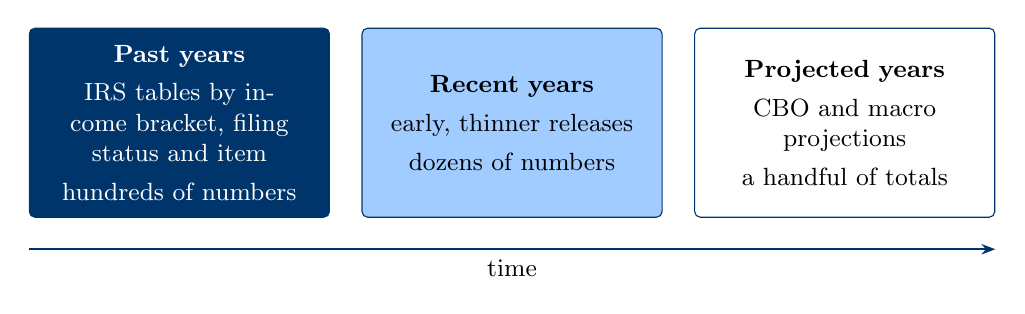
\begin{tikzpicture}
    \node[box, text width=3.6cm, minimum height=2.4cm, fill=yaleblue, text=white,
          font=\small] (past) {\textbf{Past years}\\[3pt] IRS tables by income bracket, filing status and item\\[3pt] hundreds of numbers};
    \node[box, text width=3.6cm, minimum height=2.4cm, fill=yalelight!60,
          font=\small, right=0.4cm of past] (recent) {\textbf{Recent years}\\[3pt] early, thinner releases\\[3pt] dozens of numbers};
    \node[box, text width=3.6cm, minimum height=2.4cm, fill=white,
          font=\small, right=0.4cm of recent] (future) {\textbf{Projected years}\\[3pt] CBO and macro projections\\[3pt] a handful of totals};
    \draw[arr] ($(past.south west)+(0,-0.4)$) -- node[below, font=\small, text=black] {time}
               ($(future.south east)+(0,-0.4)$);
  \end{tikzpicture}
\end{frame}

\begin{frame}{The task}
  \centering
  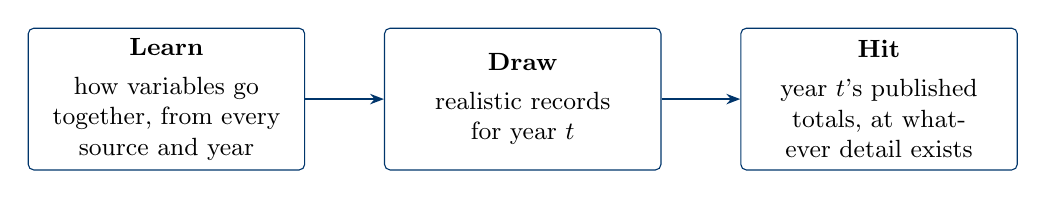
\begin{tikzpicture}
    \node[box, text width=3.3cm, minimum height=1.8cm, font=\small] (learn)
      {\textbf{Learn}\\[3pt] how variables go together, from every source and year};
    \node[box, text width=3.3cm, minimum height=1.8cm, font=\small, right=1cm of learn] (draw)
      {\textbf{Draw}\\[3pt] realistic records for year $t$};
    \node[box, text width=3.3cm, minimum height=1.8cm, font=\small, right=1cm of draw] (hit)
      {\textbf{Hit}\\[3pt] year $t$'s published totals, at whatever detail exists};
    \draw[arr] (learn) -- (draw);
    \draw[arr] (draw) -- (hit);
  \end{tikzpicture}
\end{frame}

% ===========================================================================
% 3. What we did before
% ===========================================================================

\begin{frame}{What we did before}
  \centering
  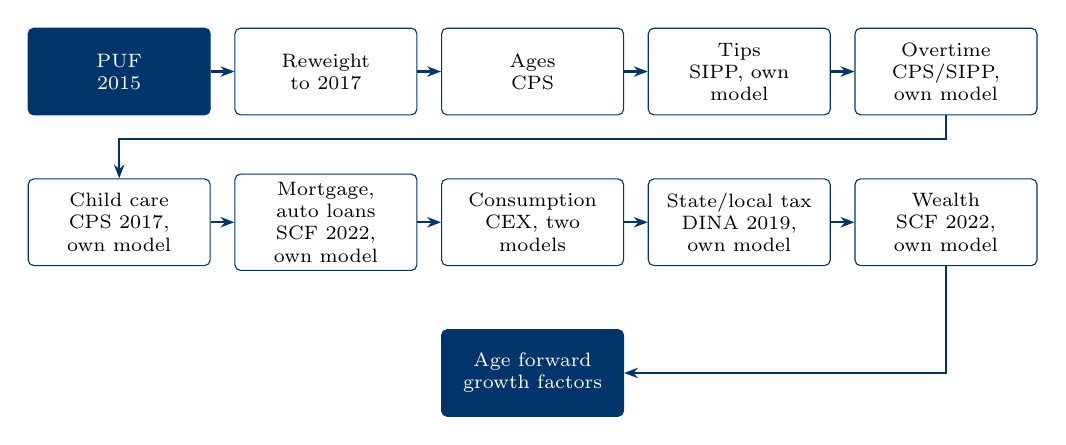
\begin{tikzpicture}[node distance=0.3cm]
    \node[box, fill=yaleblue, text=white] (a) {PUF\\2015};
    \node[box, right=of a] (b) {Reweight\\to 2017};
    \node[box, right=of b] (c) {Ages\\CPS};
    \node[box, right=of c] (d) {Tips\\SIPP, own model};
    \node[box, right=of d] (e) {Overtime\\CPS/SIPP, own model};
    \node[box, below=0.8cm of a] (f) {Child care\\CPS 2017, own model};
    \node[box, right=of f] (g) {Mortgage, auto loans\\SCF 2022, own model};
    \node[box, right=of g] (h) {Consumption\\CEX, two models};
    \node[box, right=of h] (i) {State/local tax\\DINA 2019, own model};
    \node[box, right=of i] (j) {Wealth\\SCF 2022, own model};
    \node[box, below=0.8cm of h, fill=yaleblue, text=white] (k) {Age forward\\growth factors};
    \draw[arr] (a) -- (b); \draw[arr] (b) -- (c); \draw[arr] (c) -- (d); \draw[arr] (d) -- (e);
    \draw[arr] (e.south) -- ++(0,-0.3) -| (f.north);
    \draw[arr] (f) -- (g); \draw[arr] (g) -- (h); \draw[arr] (h) -- (i); \draw[arr] (i) -- (j);
    \draw[arr] (j.south) |- (k.east);
  \end{tikzpicture}

  \vspace{0.8em}
  \begin{itemize}
    \item Each step sees only a few variables
    \item Variables come from different years: 2015, 2017, 2019, 2022
    \item Each period is aged by its own method
  \end{itemize}
\end{frame}

% ===========================================================================
% 4. The LLM analogy
% ===========================================================================

\begin{frame}{Language models: pretraining, then post-training}
  \centering
  \begin{tikzpicture}
    \begin{axis}[sentencemap, name=pre, title={\small\bfseries Pretraining}]
      \addplot3[surf, shader=interp, samples=45, domain=-3:3, y domain=-3:3]
        {1.0*g(x,y,-1.6,1.2,0.8) + 0.8*g(x,y,1.4,1.3,0.7) + 0.6*g(x,y,1.5,-1.5,0.6)
         + 0.9*g(x,y,-0.6,-0.9,0.9) + 0.5*g(x,y,0.3,0.3,0.7)};
      \maplabels{`The cat sat on the mat.'}{`Sure! Let me look\\ at your code first.'}{`The way to make\\ a bomb is'}{`mat the on cat sat'}
    \end{axis}
    \begin{axis}[sentencemap, at={($(pre.east)+(0.8cm,0)$)}, anchor=west,
        title={\small\bfseries Post-training}]
      \addplot3[surf, shader=interp, samples=45, domain=-3:3, y domain=-3:3]
        {0.2*g(x,y,-1.6,1.2,0.8) + 3.0*g(x,y,1.4,1.3,0.7) + 0.005*g(x,y,1.5,-1.5,0.6)
         + 0.2*g(x,y,-0.6,-0.9,0.9) + 0.2*g(x,y,0.3,0.3,0.7)};
      \maplabels{`The cat sat on the mat.'}{`Sure! Let me look\\ at your code first.'}{`The way to make\\ a bomb is'}{`mat the on cat sat'}
    \end{axis}
  \end{tikzpicture}

  \vspace{0.3em}
  \begin{columns}[T]
    \begin{column}{0.45\textwidth}\centering\small
      Measure how language is distributed: which sentences are likely
    \end{column}
    \begin{column}{0.45\textwidth}\centering\small
      Squeeze the mass toward the answers we want
    \end{column}
  \end{columns}
  \slidenote{Each point is a sentence; darker means more likely. Illustration.}
\end{frame}

\begin{frame}{Our model: pretraining, then post-training for 2040}
  \centering
  \begin{tikzpicture}
    \begin{axis}[sentencemap, name=pre, title={\small\bfseries Pretraining}]
      \addplot3[surf, shader=interp, samples=45, domain=-3:3, y domain=-3:3]
        {1.0*g(x,y,-1.6,1.2,0.8) + 0.8*g(x,y,1.4,1.3,0.7) + 0.6*g(x,y,1.5,-1.5,0.6)
         + 0.9*g(x,y,-0.6,-0.9,0.9) + 0.5*g(x,y,0.3,0.3,0.7)};
      \recordlabels
    \end{axis}
    \begin{axis}[sentencemap, at={($(pre.east)+(0.8cm,0)$)}, anchor=west,
        title={\small\bfseries Post-training for 2040}]
      \addplot3[surf, shader=interp, samples=45, domain=-3:3, y domain=-3:3]
        {0.5*g(x,y,-1.6,1.2,0.8) + 2.5*g(x,y,1.4,1.3,0.7) + 0.03*g(x,y,1.5,-1.5,0.6)
         + 0.6*g(x,y,-0.6,-0.9,0.9) + 0.5*g(x,y,0.3,0.3,0.7)};
      \recordlabels
    \end{axis}
  \end{tikzpicture}

  \vspace{0.3em}
  \begin{columns}[T]
    \begin{column}{0.45\textwidth}\centering\small
      Measure how tax units are distributed: which records are likely
    \end{column}
    \begin{column}{0.45\textwidth}\centering\small
      Shift the mass toward 2040: more older units, fewer retirees on 2010s interest rates
    \end{column}
  \end{columns}
  \slidenote{Each point is a tax unit; darker means more likely. Illustration.}
\end{frame}

\begin{frame}{Predicting the next word, predicting the next variable}
  \centering
  \pgfplotsset{probbars/.style={xbar, width=4.6cm, height=3.3cm, xmin=0, xmax=0.6,
      bar width=6pt, hide x axis, axis y line*=left, y axis line style={draw=none},
      ytick=data, ytick style={draw=none}, yticklabel style={font=\scriptsize},
      enlarge y limits=0.15,
      nodes near coords={\pgfmathprintnumber[fixed,precision=2,zerofill]{\pgfplotspointmeta}},
      every node near coord/.append style={font=\scriptsize}}}
  \begin{tikzpicture}
    % language row
    \node[anchor=west, font=\small\bfseries, text=yaleblue] at (0,0.8) {Language model};
    \node[tok, anchor=west] (w1) at (0,0) {`The'};
    \node[tok, right=2pt of w1] (w2) {`cat'};
    \node[tok, right=2pt of w2] (w3) {`sat'};
    \node[tok, right=2pt of w3] (w4) {`on'};
    \node[tok, right=2pt of w4] (w5) {`the'};
    \node[blank, right=2pt of w5] (w6) {?};
    \draw[arr] ($(w6.east)+(0.15,0)$) -- (8.6,0);
    \begin{axis}[probbars, at={(10.0cm,0)}, anchor=west,
        ytick={1,...,5}, yticklabels={other, `bed', `couch', `floor', `mat'}]
      \addplot[fill=yaleblue, draw=none] coordinates
        {(0.42,5) (0.15,4) (0.09,3) (0.07,2) (0.27,1)};
    \end{axis}

    % PUF row
    \node[anchor=west, font=\small\bfseries, text=yaleblue] at (0,-2.2) {Our model};
    \begin{scope}[every node/.append style={align=center, font=\scriptsize, inner sep=3pt,
                                            minimum height=1.1cm}]
      \node[tok, anchor=west] (v1) at (0,-3) {source\\PUF};
      \node[tok, right=2pt of v1] (v2) {year\\2015};
      \node[tok, right=2pt of v2] (v3) {married\\yes};
      \node[tok, right=2pt of v3] (v4) {age\\44};
      \node[tok, right=2pt of v4] (v5) {wage\\percentile\\95--96};
      \node[blank, right=2pt of v5, font=\scriptsize\bfseries] (v6) {dependents\\?};
    \end{scope}
    \draw[arr] ($(v6.east)+(0.15,0)$) -- (8.6,-3);
    \begin{axis}[probbars, at={(10.0cm,-3cm)}, anchor=west,
        ytick={1,...,4}, yticklabels={3+, 2, 1, 0}]
      \addplot[fill=yaleblue, draw=none] coordinates
        {(0.30,4) (0.20,3) (0.32,2) (0.18,1)};
    \end{axis}
  \end{tikzpicture}
  \slidenote{Made-up probabilities.}
\end{frame}

\begin{frame}{Training, step by step}
  \centering
  \begin{tikzpicture}[x=1.5cm, y=0.85cm]
    \foreach \lab [count=\i] in {source, year, married, dependents, wages, interest, dividends, net worth, UI benefits}
      \node[font=\scriptsize\bfseries, text=yaleblue, text depth=0.3ex] at (\i, -0.2) {\lab};
    \foreach \src/\yr [count=\r] in {PUF/2015, PUF/2015, SCF/2019, SCF/2016} {
      \node[cell] at (1,-\r) {\src};
      \node[cell] at (2,-\r) {\yr};
    }
    \only<1>{%
      \node[font=\small] at (5,0.75) {Training data: real records from the PUF and the SCF};
      \cellv{3}{1}{yes} \cellv{4}{1}{2} \cellv{5}{1}{\$142k} \cellv{6}{1}{\$310} \cellv{7}{1}{\$2.4k} \cella{8}{1} \cellv{9}{1}{\$0}
      \cellv{3}{2}{no} \cellv{4}{2}{0} \cellv{5}{2}{\$38k} \cellv{6}{2}{\$0} \cellv{7}{2}{\$0} \cella{8}{2} \cellv{9}{2}{\$4.2k}
      \cellv{3}{3}{no} \cellv{4}{3}{1} \cellv{5}{3}{\$48k} \cellv{6}{3}{\$120} \cellv{7}{3}{\$0} \cellv{8}{3}{\$85k} \cella{9}{3}
      \cellv{3}{4}{yes} \cellv{4}{4}{2} \cellv{5}{4}{\$95k} \cellv{6}{4}{\$350} \cellv{7}{4}{\$1.1k} \cellv{8}{4}{\$610k} \cella{9}{4}
      \trainnet{idle}
    }
    \only<2>{%
      \node[font=\small] at (5,0.75) {Hide a random set of cells (source and year always stay visible)};
      \cellv{3}{1}{yes} \cellh{4}{1} \cellv{5}{1}{\$142k} \cellh{6}{1} \cellv{7}{1}{\$2.4k} \cella{8}{1} \cellv{9}{1}{\$0}
      \cellh{3}{2} \cellv{4}{2}{0} \cellh{5}{2} \cellv{6}{2}{\$0} \cellv{7}{2}{\$0} \cella{8}{2} \cellh{9}{2}
      \cellv{3}{3}{no} \cellv{4}{3}{1} \cellv{5}{3}{\$48k} \cellh{6}{3} \cellv{7}{3}{\$0} \cellh{8}{3} \cella{9}{3}
      \cellv{3}{4}{yes} \cellv{4}{4}{2} \cellh{5}{4} \cellv{6}{4}{\$350} \cellv{7}{4}{\$1.1k} \cellv{8}{4}{\$610k} \cella{9}{4}
      \trainnet{idle}
    }
    \only<3>{%
      \node[font=\small] at (5,0.75) {The network guesses a distribution for each hidden cell};
      \cellv{3}{1}{yes} \cellg{4}{1}{0.66,0.79,0.72,0.82}{0}{2} \cellv{5}{1}{\$142k} \cellg{6}{1}{0.83,0.58,0.56,0.93,0.67}{0}{\$310} \cellv{7}{1}{\$2.4k} \cella{8}{1} \cellv{9}{1}{\$0}
      \cellg{3}{2}{0.66,1.00}{0}{no} \cellv{4}{2}{0} \cellg{5}{2}{0.76,0.93,0.76,0.84,0.62}{0}{\$38k} \cellv{6}{2}{\$0} \cellv{7}{2}{\$0} \cella{8}{2} \cellg{9}{2}{0.84,0.94,0.79,0.88,0.85}{0}{\$4.2k}
      \cellv{3}{3}{no} \cellv{4}{3}{1} \cellv{5}{3}{\$48k} \cellg{6}{3}{0.58,0.89,0.82,0.69,0.56}{0}{\$120} \cellv{7}{3}{\$0} \cellg{8}{3}{0.94,0.76,0.87,0.95,0.87}{0}{\$85k} \cella{9}{3}
      \cellv{3}{4}{yes} \cellv{4}{4}{2} \cellg{5}{4}{0.96,0.73,0.91,0.75,0.97}{0}{\$95k} \cellv{6}{4}{\$350} \cellv{7}{4}{\$1.1k} \cellv{8}{4}{\$610k} \cella{9}{4}
      \trainnet{guess}
    }
    \only<4>{%
      \node[font=\small] at (5,0.75) {Compare with the truth (dark bar)};
      \cellv{3}{1}{yes} \cellg{4}{1}{0.66,0.79,0.72,0.82}{3}{2} \cellv{5}{1}{\$142k} \cellg{6}{1}{0.83,0.58,0.56,0.93,0.67}{2}{\$310} \cellv{7}{1}{\$2.4k} \cella{8}{1} \cellv{9}{1}{\$0}
      \cellg{3}{2}{0.66,1.00}{2}{no} \cellv{4}{2}{0} \cellg{5}{2}{0.76,0.93,0.76,0.84,0.62}{3}{\$38k} \cellv{6}{2}{\$0} \cellv{7}{2}{\$0} \cella{8}{2} \cellg{9}{2}{0.84,0.94,0.79,0.88,0.85}{3}{\$4.2k}
      \cellv{3}{3}{no} \cellv{4}{3}{1} \cellv{5}{3}{\$48k} \cellg{6}{3}{0.58,0.89,0.82,0.69,0.56}{2}{\$120} \cellv{7}{3}{\$0} \cellg{8}{3}{0.94,0.76,0.87,0.95,0.87}{3}{\$85k} \cella{9}{3}
      \cellv{3}{4}{yes} \cellv{4}{4}{2} \cellg{5}{4}{0.96,0.73,0.91,0.75,0.97}{4}{\$95k} \cellv{6}{4}{\$350} \cellv{7}{4}{\$1.1k} \cellv{8}{4}{\$610k} \cella{9}{4}
      \node[font=\scriptsize, text=yaleblue, anchor=east, align=right] at (9.6,-5.5) {probability on the truth: 0.21};
      \trainnet{guess}
    }
    \only<5>{%
      \node[font=\small] at (5,0.75) {Nudge every weight so the truth gets more probability};
      \cellv{3}{1}{yes} \cellg{4}{1}{0.66,0.79,0.72,0.82}{3}{2} \cellv{5}{1}{\$142k} \cellg{6}{1}{0.83,0.58,0.56,0.93,0.67}{2}{\$310} \cellv{7}{1}{\$2.4k} \cella{8}{1} \cellv{9}{1}{\$0}
      \cellg{3}{2}{0.66,1.00}{2}{no} \cellv{4}{2}{0} \cellg{5}{2}{0.76,0.93,0.76,0.84,0.62}{3}{\$38k} \cellv{6}{2}{\$0} \cellv{7}{2}{\$0} \cella{8}{2} \cellg{9}{2}{0.84,0.94,0.79,0.88,0.85}{3}{\$4.2k}
      \cellv{3}{3}{no} \cellv{4}{3}{1} \cellv{5}{3}{\$48k} \cellg{6}{3}{0.58,0.89,0.82,0.69,0.56}{2}{\$120} \cellv{7}{3}{\$0} \cellg{8}{3}{0.94,0.76,0.87,0.95,0.87}{3}{\$85k} \cella{9}{3}
      \cellv{3}{4}{yes} \cellv{4}{4}{2} \cellg{5}{4}{0.96,0.73,0.91,0.75,0.97}{4}{\$95k} \cellv{6}{4}{\$350} \cellv{7}{4}{\$1.1k} \cellv{8}{4}{\$610k} \cella{9}{4}
      \node[font=\scriptsize, text=yaleblue, anchor=east, align=right] at (9.6,-5.5) {update 1\\probability on the truth: 0.21};
      \trainnet{update}
    }
    \only<6>{%
      \node[font=\small] at (5,0.75) {Next batch: hide a different random set};
      \cellv{3}{1}{yes} \cellv{4}{1}{2} \cellh{5}{1} \cellv{6}{1}{\$310} \cellh{7}{1} \cella{8}{1} \cellh{9}{1}
      \cellv{3}{2}{no} \cellh{4}{2} \cellv{5}{2}{\$38k} \cellv{6}{2}{\$0} \cellv{7}{2}{\$0} \cella{8}{2} \cellv{9}{2}{\$4.2k}
      \cellh{3}{3} \cellv{4}{3}{1} \cellh{5}{3} \cellv{6}{3}{\$120} \cellv{7}{3}{\$0} \cellv{8}{3}{\$85k} \cella{9}{3}
      \cellv{3}{4}{yes} \cellv{4}{4}{2} \cellv{5}{4}{\$95k} \cellh{6}{4} \cellv{7}{4}{\$1.1k} \cellh{8}{4} \cella{9}{4}
      \trainnet{idle}
    }
    \only<7>{%
      \node[font=\small] at (5,0.75) {Guess, compare, nudge again};
      \cellv{3}{1}{yes} \cellv{4}{1}{2} \cellg{5}{1}{0.65,0.34,0.35,1.00,0.39}{4}{\$142k} \cellv{6}{1}{\$310} \cellg{7}{1}{0.69,0.47,1.00,0.55,0.42}{3}{\$2.4k} \cella{8}{1} \cellg{9}{1}{1.00,0.50,0.45,0.44,0.53}{1}{\$0}
      \cellv{3}{2}{no} \cellg{4}{2}{1.00,0.53,0.66,0.57}{1}{0} \cellv{5}{2}{\$38k} \cellv{6}{2}{\$0} \cellv{7}{2}{\$0} \cella{8}{2} \cellv{9}{2}{\$4.2k}
      \cellg{3}{3}{0.67,1.00}{2}{no} \cellv{4}{3}{1} \cellg{5}{3}{0.64,0.70,1.00,0.57,0.37}{3}{\$48k} \cellv{6}{3}{\$120} \cellv{7}{3}{\$0} \cellv{8}{3}{\$85k} \cella{9}{3}
      \cellv{3}{4}{yes} \cellv{4}{4}{2} \cellv{5}{4}{\$95k} \cellg{6}{4}{0.64,1.00,0.69,0.66,0.53}{2}{\$350} \cellv{7}{4}{\$1.1k} \cellg{8}{4}{0.59,0.38,0.63,1.00,0.53}{4}{\$610k} \cella{9}{4}
      \node[font=\scriptsize, text=yaleblue, anchor=east, align=right] at (9.6,-5.5) {update 2\\probability on the truth: 0.27};
      \trainnet{update}
    }
    \only<8>{%
      \node[font=\small] at (5,0.75) {After about 10,000 updates, 4,096 records each};
      \cellg{3}{1}{1.00,0.08}{1}{yes} \cellv{4}{1}{2} \cellv{5}{1}{\$142k} \cellg{6}{1}{0.05,1.00,0.16,0.18,0.05}{2}{\$310} \cellv{7}{1}{\$2.4k} \cella{8}{1} \cellv{9}{1}{\$0}
      \cellv{3}{2}{no} \cellv{4}{2}{0} \cellv{5}{2}{\$38k} \cellv{6}{2}{\$0} \cellg{7}{2}{1.00,0.15,0.10,0.06,0.08}{1}{\$0} \cella{8}{2} \cellg{9}{2}{0.15,0.16,1.00,0.05,0.13}{3}{\$4.2k}
      \cellv{3}{3}{no} \cellg{4}{3}{0.05,1.00,0.14,0.09}{2}{1} \cellv{5}{3}{\$48k} \cellv{6}{3}{\$120} \cellv{7}{3}{\$0} \cellg{8}{3}{0.16,0.18,1.00,0.11,0.18}{3}{\$85k} \cella{9}{3}
      \cellv{3}{4}{yes} \cellg{4}{4}{0.08,0.05,1.00,0.12}{3}{2} \cellv{5}{4}{\$95k} \cellv{6}{4}{\$350} \cellg{7}{4}{0.04,0.07,1.00,0.10,0.13}{3}{\$1.1k} \cellv{8}{4}{\$610k} \cella{9}{4}
      \node[font=\scriptsize, text=yaleblue, anchor=east, align=right] at (9.6,-5.5) {probability on the truth: 0.74};
      \trainnet{guess}
    }
  \end{tikzpicture}
  \slidenote{Made-up records and numbers.}
\end{frame}

\begin{frame}{Training: fill in the blanks}
  \begin{itemize}
    \item Hide, guess, compare, nudge: about 10,000 times
    \vspace{0.4em}
    \item The blanks can be anywhere, so one model answers every question
          of the form ``this variable, given those''
    \vspace{0.4em}
    \item A variable a source never has (grey: net worth on the PUF, UI benefits on the SCF) is never asked
  \end{itemize}
\end{frame}

\begin{frame}{Writing a record, one variable at a time}
  \centering
  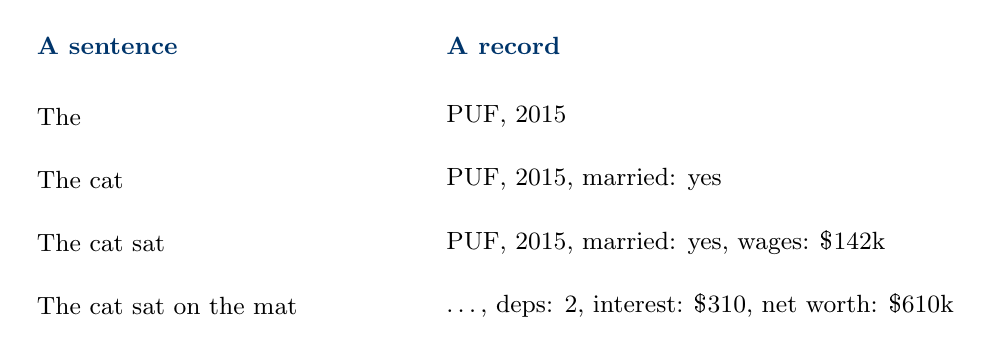
\begin{tikzpicture}
    \foreach \y/\txt in {0/The, 1/The cat, 2/The cat sat, 3/The cat sat on the mat} {
      \node[anchor=west, font=\small] at (0, -\y*0.8) {\txt};
    }
    \node[anchor=west, font=\small\bfseries, text=yaleblue] at (0, 0.9) {A sentence};

    \foreach \y/\txt in {0/{PUF, 2015},
                         1/{PUF, 2015, married: yes},
                         2/{PUF, 2015, married: yes, wages: \$142k},
                         3/{\dots, deps: 2, interest: \$310, net worth: \$610k}} {
      \node[anchor=west, font=\small] at (5.2, -\y*0.8) {\txt};
    }
    \node[anchor=west, font=\small\bfseries, text=yaleblue] at (5.2, 0.9) {A record};
  \end{tikzpicture}

  \vspace{1.2em}
  Each step: ask the model for the probabilities, draw one, add it to the context.
  \slidenote{Made-up records.}
\end{frame}

\begin{frame}{Why deep learning}
  \begin{itemize}
    \item \textbf{One model, every question.} No chain of separate imputations.
    \vspace{0.4em}
    \item \textbf{It finds the interactions itself.} Nonlinear, many variables at once.
    \vspace{0.4em}
    \item \textbf{Gaps are just blanks.} Every source trains the same model, whatever it is missing.
    \vspace{0.4em}
    \item \textbf{Source and year are part of the prompt.} Ask for a record ``as the 2015 PUF would show it'' or ``as the 2019 SCF would''.
  \end{itemize}
\end{frame}

% ===========================================================================
% 5. Post-training
% ===========================================================================

\begin{frame}{Post-training: hit the totals}
  \centering
  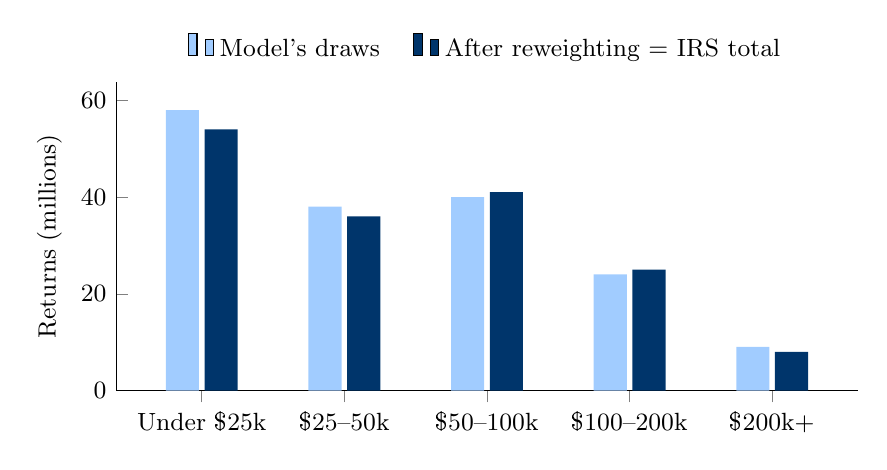
\begin{tikzpicture}
    \begin{axis}[ybar, width=11cm, height=5.5cm, bar width=12pt, ymin=0,
        symbolic x coords={Under \$25k, \$25--50k, \$50--100k, \$100--200k, \$200k+},
        xtick=data, xticklabel style={font=\small}, ylabel={Returns (millions)},
        ylabel style={font=\small}, yticklabel style={font=\small},
        legend style={font=\small, draw=none, at={(0.5,1.03)}, anchor=south, legend columns=2,
                      /tikz/every even column/.append style={column sep=1em}},
        axis x line*=bottom, axis y line*=left, enlarge x limits=0.15]
      \addplot[fill=yalelight!60, draw=none] coordinates
        {(Under \$25k,58) (\$25--50k,38) (\$50--100k,40) (\$100--200k,24) (\$200k+,9)};
      \addplot[fill=yaleblue, draw=none] coordinates
        {(Under \$25k,54) (\$25--50k,36) (\$50--100k,41) (\$100--200k,25) (\$200k+,8)};
      \legend{Model's draws, After reweighting = IRS total}
    \end{axis}
  \end{tikzpicture}

  \vspace{0.3em}
  Change the weights as little as possible while matching every total.
  \slidenote{Made-up numbers.}
\end{frame}

% ===========================================================================
% 6. Challenges
% ===========================================================================

\begin{frame}{Challenge: the same word means different things}
  \centering
  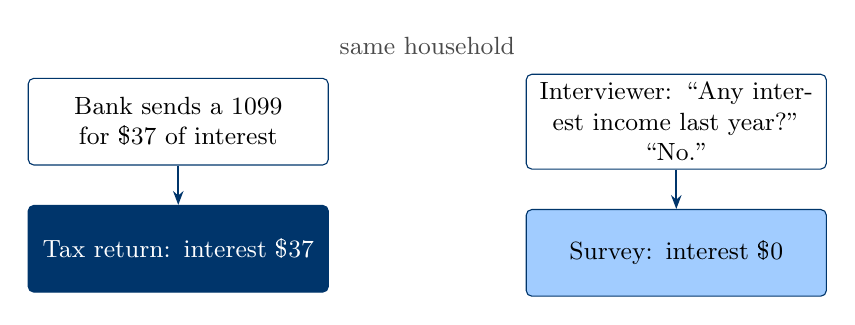
\begin{tikzpicture}
    \node[box, text width=3.6cm, font=\small] (bank) {Bank sends a 1099 for \$37 of interest};
    \node[box, text width=3.6cm, font=\small, below=0.5cm of bank, fill=yaleblue, text=white] (puf) {Tax return: interest \$37};
    \node[box, text width=3.6cm, font=\small, right=2.5cm of bank] (ask) {Interviewer: ``Any interest income last year?'' \\ ``No.''};
    \node[box, text width=3.6cm, font=\small, below=0.5cm of ask, fill=yalelight!60] (scf) {Survey: interest \$0};
    \draw[arr] (bank) -- (puf);
    \draw[arr] (ask) -- (scf);
    \node[font=\small, text=yalegrey, above=0.15cm] at ($(bank.north)!0.5!(ask.north)$) {same household};
  \end{tikzpicture}

  \vspace{1em}
  \begin{tabular}{ll}
    \textbf{Population}  & filers or everyone; tax units or households \\
    \textbf{Definition}  & what counts: e.g.\ losses capped at \$3,000 on a return \\
    \textbf{Measurement} & small amounts forgotten, misremembered, rounded \\
  \end{tabular}
\end{frame}

% Translation, worked through SCF interest. Real numbers: 2016 SCF (tax year
% 2015) against the 2015 PUF, weighted, per 100 tax units, married with wages
% $75k-200k. Source: rebuild/explore/2026-10-21/reporting_formula/
% check_consistent_seed20261016/report.md (columns "data" and "cell target").

\begin{frame}{Interest: how many hold any?}
  \centering
  \begin{tikzpicture}
    \begin{axis}[ybar, width=12cm, height=5.4cm, bar width=14pt, ymin=0, ymax=32,
        symbolic x coords={\$1--100, \$100--500, \$500--2k, \$2k--10k, \$10k+},
        xtick=data, xticklabel style={font=\small}, yticklabel style={font=\small},
        ylabel={Per 100 tax units}, ylabel style={font=\small},
        xlabel={Interest received in the year}, xlabel style={font=\small},
        legend style={font=\small, draw=none, at={(0.97,0.95)}, anchor=north east},
        axis x line*=bottom, axis y line*=left, enlarge x limits=0.12,
        nodes near coords, every node near coord/.append style={font=\scriptsize}]
      \addplot[fill=yaleblue, draw=none] coordinates
        {(\$1--100,28) (\$100--500,13) (\$500--2k,4) (\$2k--10k,2) (\$10k+,1)};
      \addplot[fill=yalelight!70, draw=none] coordinates
        {(\$1--100,8) (\$100--500,6) (\$500--2k,3) (\$2k--10k,3) (\$10k+,1)};
      \legend{PUF: on the return (48 in all), SCF: say they have it (21 in all)}
    \end{axis}
  \end{tikzpicture}

  \vspace{0.3em}
  The gap is all in small amounts. Above \$2,000 the two sources agree.
  \slidenote{Married, wages \$75--200k. 2015 PUF and 2016 SCF (tax year 2015), weighted.}
\end{frame}

\begin{frame}{Small amounts go unreported}
  \centering
  \begin{tikzpicture}
    \begin{axis}[ybar, width=11cm, height=5.2cm, bar width=22pt, ymin=0, ymax=150,
        symbolic x coords={\$1--100, \$100--500, \$500--2k, \$2k+},
        xtick=data, xticklabel style={font=\small}, yticklabel style={font=\small},
        ylabel={SCF reporters per 100 PUF holders}, ylabel style={font=\small},
        axis x line*=bottom, axis y line*=left, enlarge x limits=0.15,
        nodes near coords, every node near coord/.append style={font=\small}]
      \addplot[fill=yaleblue, draw=none] coordinates
        {(\$1--100,30) (\$100--500,48) (\$500--2k,61) (\$2k+,135)};
      \draw[dashed, yalegrey] (rel axis cs:0,0.667) -- node[pos=0.02, above, font=\scriptsize, anchor=south west] {as many as the PUF} (rel axis cs:1,0.667);
    \end{axis}
  \end{tikzpicture}

  \vspace{0.3em}
  Of every 100 couples whose return shows \$1--100 of interest,\\
  only about 30 tell the SCF they have any.
  \slidenote{Married, wages \$75--200k. 2015 PUF, 2016 SCF, weighted. Above 100: no fill-in.}
\end{frame}

\begin{frame}{Why it matters: what interest says about wealth}
  \centering
  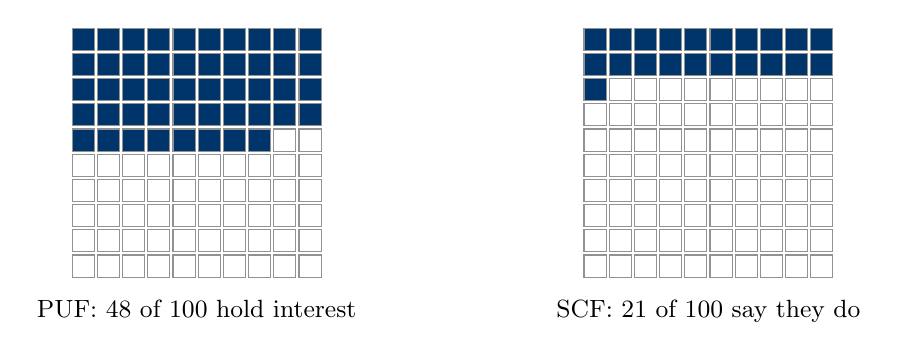
\begin{tikzpicture}
    \waffle{0,0}{48}{0}{PUF: 48 of 100 hold interest}
    \waffle{6.5,0}{21}{0}{SCF: 21 of 100 say they do}
  \end{tikzpicture}

  \vspace{0.8em}
  \small
  \begin{itemize}
    \item Wealth comes only from the SCF: the model learns what interest holders own from the 21
    \item It then applies that to the PUF's 48. But the 21 lean toward larger amounts
    \item In our first test, taking SCF answers at face value put net worth off by a factor of two
  \end{itemize}
  \slidenote{Married, wages \$75--200k. 2015 PUF and 2016 SCF, weighted.}
\end{frame}

\begin{frame}{The fix, step 1: two slots}
  \centering
  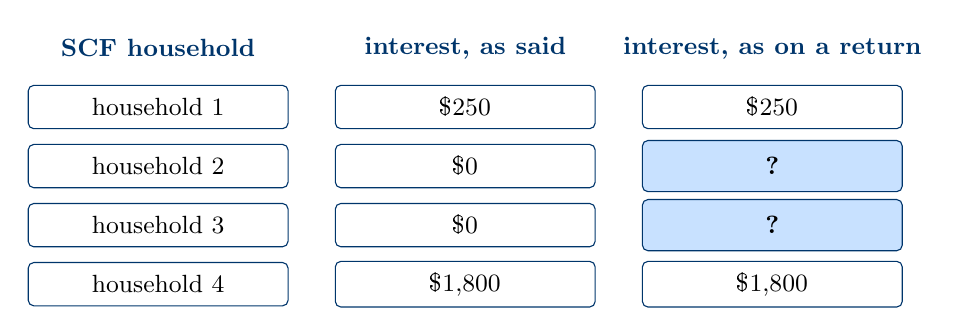
\begin{tikzpicture}[x=3.9cm, y=0.75cm,
      c/.style={tok, minimum width=3.3cm, minimum height=0.55cm, font=\small}]
    \node[font=\small\bfseries, text=yaleblue] at (1,0) {SCF household};
    \node[font=\small\bfseries, text=yaleblue] at (2,0) {interest, as said};
    \node[font=\small\bfseries, text=yaleblue] at (3,0) {interest, as on a return};
    \foreach \r/\said/\ret/\hd in {1/\$250/\$250/0, 2/\$0/?/1, 3/\$0/?/1, 4/{\$1,800}/{\$1,800}/0} {
      \node[c] at (1,-\r) {household \r};
      \node[c] at (2,-\r) {\said};
      \ifnum\hd=1 \node[c, blank] at (3,-\r) {\ret}; \else \node[c] at (3,-\r) {\ret}; \fi
    }
  \end{tikzpicture}

  \vspace{0.6em}
  \small
  \begin{itemize}
    \item The answer the household gave is kept, never changed
    \item A second slot holds what its tax return would show
    \item Reporters copy their answer. Zero-reporters get filled in, some with a small amount
    \item PUF records have only the second slot, so both sources now mean the same thing by ``interest''
  \end{itemize}
\end{frame}

\begin{frame}{The fix, step 2: how many to fill in}
  \begin{columns}[c]
    \begin{column}{0.42\textwidth}
      \centering
      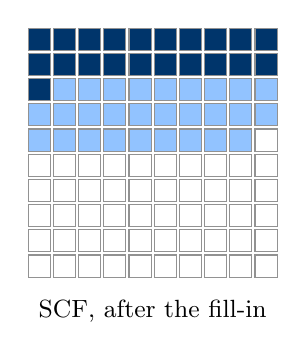
\begin{tikzpicture}
        \waffle{0,0}{21}{28}{SCF, after the fill-in}
      \end{tikzpicture}

      \vspace{0.5em}
      {\scriptsize
      \tikz\fill[yaleblue] (0,0) rectangle (0.2,0.2); reported \quad
      \tikz\fill[yalelight!70] (0,0) rectangle (0.2,0.2); filled in \quad
      \tikz\draw[yalegrey] (0,0) rectangle (0.2,0.2); none}
    \end{column}
    \begin{column}{0.55\textwidth}
      \small
      \begin{tabular}{lrrr}
        \toprule
        Per 100 couples & PUF & SCF & Fill in \\
        \midrule
        \$1--100      & 28 & 8 & 20 \\
        \$100--500    & 13 & 6 & 7 \\
        \$500--2k     & 4  & 3 & 2 \\
        \$2k and over & 3  & 3 & 0 \\
        \midrule
        Any           & 48 & 21 & 28 \\
        \bottomrule
      \end{tabular}

      \vspace{1em}
      The PUF says how many hidden holders there are, and at what sizes.
      Of the 79 couples who said none, about 28 get a small amount.
    \end{column}
  \end{columns}
  \slidenote{Married, wages \$75--200k. 2015 PUF and 2016 SCF, weighted. Rows may not add because of rounding.}
\end{frame}

\begin{frame}{The fix, step 3: which households}
  For \$1--100: 30 report for every 100 holders, so each reporter stands for\\
  $100/30 - 1 \approx 2.3$ hidden holders.

  \vspace{0.8em}
  \begin{columns}[T]
    \begin{column}{0.47\textwidth}
      \begin{block}{Couple A: said no interest}
        \$300k in the bank, owns stocks\\[3pt]
        Model: looks like a reporter of \$1--100 with chance 20\%, like a zero with 60\%\\[3pt]
        Chance of a hidden holding:\\
        $20\% \times 2.3 \div 60\% \approx$ \textbf{78\%}
      \end{block}
    \end{column}
    \begin{column}{0.47\textwidth}
      \begin{block}{Couple B: said no interest}
        \$3k net worth, renter\\[3pt]
        Model: looks like a reporter of \$1--100 with chance 2\%, like a zero with 95\%\\[3pt]
        Chance of a hidden holding:\\
        $2\% \times 2.3 \div 95\% \approx$ \textbf{5\%}
      \end{block}
    \end{column}
  \end{columns}

  \vspace{0.6em}
  Households that look like reporters get most of the fill-ins. The PUF sets how many;
  the rest of the SCF record sets who.
  \slidenote{Couples A and B are made up; the 30 per 100 is real.}
\end{frame}

\begin{frame}{The fix, step 4: inside training}
  \begin{columns}[c]
    \begin{column}{0.5\textwidth}
      \centering
      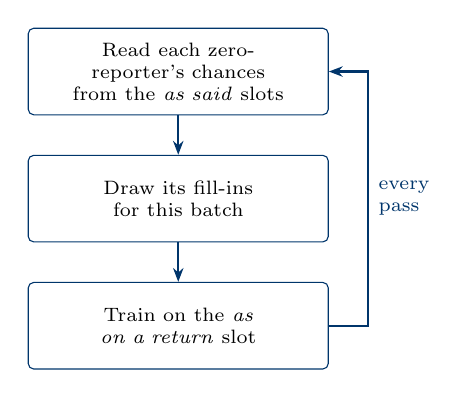
\begin{tikzpicture}[node distance=0.5cm]
        \node[box, text width=3.6cm] (a) {Read each zero-reporter's chances from the \emph{as said} slots};
        \node[box, text width=3.6cm, below=of a] (b) {Draw its fill-ins for this batch};
        \node[box, text width=3.6cm, below=of b] (c) {Train on the \emph{as on a return} slot};
        \draw[arr] (a) -- (b);
        \draw[arr] (b) -- (c);
        \draw[arr] (c.east) -- ++(0.5,0) |- node[pos=0.25, right, font=\scriptsize, align=left] {every\\pass} (a.east);
      \end{tikzpicture}
    \end{column}
    \begin{column}{0.48\textwidth}
      \centering
      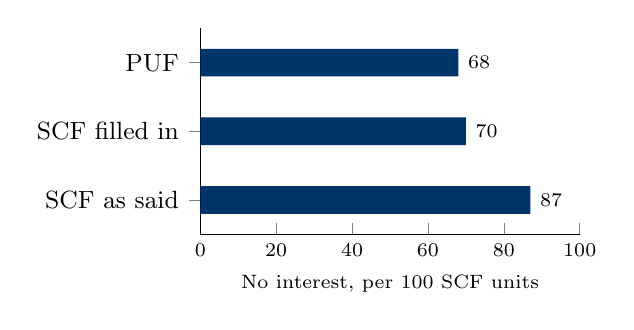
\begin{tikzpicture}
        \begin{axis}[xbar, width=6.4cm, height=4.2cm, bar width=10pt, xmin=0, xmax=100,
            ytick={1,2,3}, yticklabels={SCF as said, SCF filled in, PUF},
            yticklabel style={font=\small}, xticklabel style={font=\scriptsize},
            xlabel={No interest, per 100 SCF units}, xlabel style={font=\scriptsize},
            axis x line*=bottom, axis y line*=left, enlarge y limits=0.25,
            nodes near coords, every node near coord/.append style={font=\scriptsize}]
          \addplot[fill=yaleblue, draw=none] coordinates {(87,1) (70,2) (68,3)};
        \end{axis}
      \end{tikzpicture}
    \end{column}
  \end{columns}

  \vspace{0.6em}
  The fill-ins never feed back into the chances, so the model does not learn from its own guesses.
  \slidenote{2016 SCF units (tax year 2015); PUF predicted at the same household types. Latest model, 21 October.}
\end{frame}

\begin{frame}{What the fix assumes, and how well it works}
  \begin{block}{The assumption}
    Whether a holder reports depends only on its type (married, dependents, wages)
    and how much it holds. Nothing else on the record.
  \end{block}

  \vspace{0.3em}
  \begin{block}{A test with a known answer}
    Make PUF records answer the way SCF households do, then try to undo it.
    \begin{itemize}
      \item True share with no interest: 71.6\%. Recovered: 70.7--73.0\%
      \item If reporting also depends on something the record does not show,
            it overcorrects by about 8\%
    \end{itemize}
  \end{block}

  \vspace{0.3em}
  \begin{block}{On the real SCF}
    Still about 1.7 points short of the PUF for interest: some households come out
    with a chance above 100\%, and are capped
  \end{block}
\end{frame}

\begin{frame}{Challenge: the return itself changes}
  \begin{columns}[c]
    \begin{column}{0.45\textwidth}
      \centering
      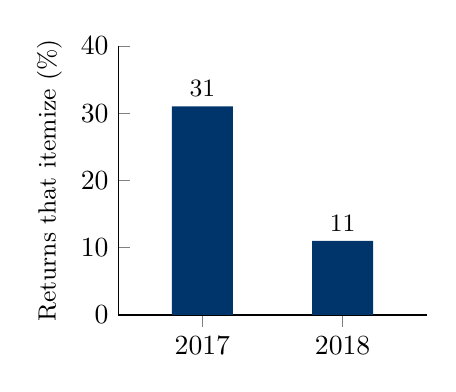
\begin{tikzpicture}
        \begin{axis}[ybar, width=5.5cm, height=5cm, bar width=22pt, ymin=0, ymax=40,
            symbolic x coords={2017,2018}, xtick=data, enlarge x limits=0.6,
            ylabel={Returns that itemize (\%)}, ylabel style={font=\small},
            axis x line*=bottom, axis y line*=left, nodes near coords,
            every node near coord/.append style={font=\small}]
          \addplot[fill=yaleblue, draw=none] coordinates {(2017,31) (2018,11)};
        \end{axis}
      \end{tikzpicture}
    \end{column}
    \begin{column}{0.52\textwidth}
      \begin{itemize}
        \item The 2017 tax law cut itemizing by two thirds
        \item A 2015 return shows mortgage interest for people who no longer report it
        \item New items, like the tips and overtime deductions, are on no past return
      \end{itemize}
    \end{column}
  \end{columns}
  \slidenote{Approximate shares.}
\end{frame}

\begin{frame}{Other challenges}
  \begin{columns}[T]
    \begin{column}{0.48\textwidth}
      \begin{block}{Different populations}
        The PUF has no non-filers. Surveys count households, not tax units.
      \end{block}
      \begin{block}{A thin top}
        Few very rich records in any source.
      \end{block}
    \end{column}
    \begin{column}{0.48\textwidth}
      \begin{block}{Future years}
        No microdata. Only targets, and a choice of which past years to lean on.
      \end{block}
      \begin{block}{Checking the result}
        No source has every variable, so some relationships have no truth to compare against.
      \end{block}
    \end{column}
  \end{columns}
\end{frame}

% ===========================================================================
% 7. Where we are
% ===========================================================================

\begin{frame}{Where we are}
  \begin{itemize}
    \item A 2019 file: every PUF variable plus a 20-item balance sheet
    \item Trained on the 2015 PUF and four SCF waves (2013--2022)
    \item Hits about 285 targets: IRS by income bracket, IRS business income, SCF wealth
    \item Median net worth \$90,900 against the SCF's \$91,050
  \end{itemize}
\end{frame}

\begin{frame}{What is left}
  \begin{itemize}
    \item More surveys: CPS, CEX, SIPP
    \item Projected years
    \item A tax calculator inside post-training, for targets on computed tax
    \item A standing set of checks
    \item Replace the current pipeline as Tax-Simulator's input
  \end{itemize}
\end{frame}

\begin{frame}[plain,noframenumbering,c]
  \begin{center}
    {\color{yaleblue}\Large\bfseries Questions}
  \end{center}
\end{frame}

\end{document}
